\section{FreeDOS}

\subsection{Nombre del proyecto o sistema operativo}
El sistema operativo FreeDOS, su nombre proviene de la idea de ofrecer una alternativa libre y abierta al sistema operativo MS-DOS, tras el anuncio de Microsoft en 1994 de interrumpir el soporte a este último \citep{freedos_home}.  

\subsection{Enlace al repositorio y/o documentación oficial}
\begin{itemize}
    \item \textbf{Repositorio oficial:} \url{https://github.com/FDOS}
    \item \textbf{Sitio web del proyecto:} \url{https://www.freedos.org/}
\end{itemize}

\subsection{Objetivo del proyecto}
El objetivo principal de FreeDOS es proporcionar un sistema operativo compatible con MS-DOS completamente libre, de código abierto y mantenido por la comunidad.  
Busca preservar la capacidad de ejecutar aplicaciones y controladores diseñados originalmente para DOS, especialmente aquellas dependientes de entornos de 16 bits \citep{freedos_home}.  

\subsection{Lenguaje(s) de implementación}
FreeDOS está desarrollado principalmente en \texttt{C}, con secciones escritas en \texttt{x86 Assembly}, especialmente en el núcleo y los controladores de dispositivo.  
El lenguaje C se utiliza para la lógica general del sistema, mientras que el ensamblador proporciona control de bajo nivel sobre interrupciones, rutinas BIOS y gestión de hardware.  
Este enfoque híbrido permite combinar eficiencia y compatibilidad con el hardware x86, tal como lo hacía MS-DOS \citep{freedos_developers}.  

\subsection{Arquitectura del sistema}
FreeDOS hereda la arquitectura clásica de MS-DOS, organizada en capas que separan el hardware del usuario mediante el BIOS y un núcleo DOS.  
El sistema se ejecuta en modo real (16 bits), operando directamente sobre la arquitectura Intel x86 sin protección de memoria ni multitarea.  

Se presenta un esquema adaptado que representa la arquitectura del sistema operativo MS-DOS en que se basa FreeDOS.

\begin{figure}[H]
\centering
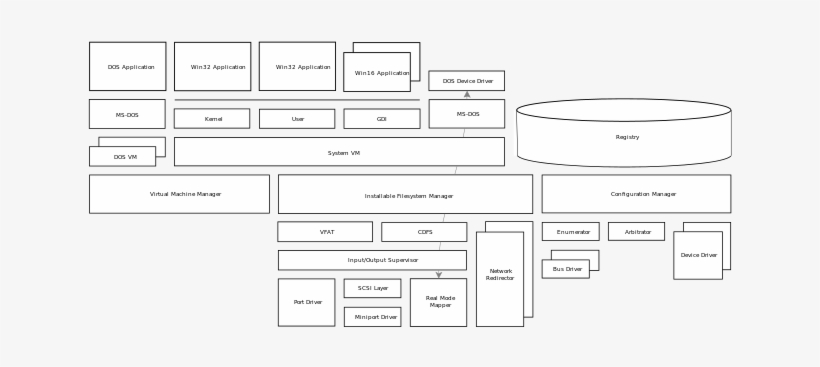
\includegraphics[width=0.9\textwidth]{figures/architecturefreedos.png}
\caption{Arquitectura clásica de MS-DOS, base de FreeDOS.}
\label{fig:freedos_architecture}
\centering
\small Fuente: Adaptado de Microsoft Press, \citep{msdos_architecture_diagram}, \textit{FreeDOS Kernel: An MS-DOS Emulator} (1996).
\end{figure}
